% Author:Zhuming Shi, Peking University
% Theme from https://github.com/matze/mtheme

% \documentclass[12pt,AutoFakeBold,aspectratio=169,mathserif]{beamer}
\documentclass[AutoFakeBold]{beamer}
\usepackage[english]{babel}

\usetheme{metropolis}

\usepackage{fontspec}% 控制字体
\setmainfont{Times New Roman}% 英文字体
\newfontfamily\arial{Arial}% Arial字体

\usepackage{xeCJK} % 中文支持
\setCJKmainfont{SimHei} % 中文字体
\XeTeXlinebreaklocale "zh"%中文自动换行
\XeTeXlinebreakskip = 0pt plus 1pt%中文自动换行

\usepackage{graphicx}
\usepackage{subfigure}
\usepackage{caption}

\usepackage{amsthm,amsmath,amssymb,mathrsfs}% 数学符号和花体支持
\usepackage{booktabs}% 绘制三线表
\usepackage{latexsym}% 绘制特殊数学符号
\usepackage{siunitx}% 数学模式中使用SI单位

\usepackage[version=3]{mhchem}% 化学反应式
\usepackage{epstopdf}% 插入ChemDraw的.eps结构图

% 代码环境
\usepackage{listings}
\usepackage{color}

\definecolor{dkgreen}{rgb}{0,0.6,0}
\definecolor{gray}{rgb}{0.5,0.5,0.5}
\definecolor{mauve}{rgb}{0.58,0,0.82}

\lstset{frame=tb,
  language=c++,
  aboveskip=3mm,
  belowskip=3mm,
  showstringspaces=false,
  columns=flexible,
  basicstyle={\small\ttfamily},
  numbers=none,
  numberstyle=\tiny\color{gray},
  keywordstyle=\color{blue},
  commentstyle=\color{dkgreen},
  stringstyle=\color{mauve},
  breaklines=true,
  breakatwhitespace=true,
  tabsize=3
}

\setbeamerfont{footnote}{size=\tiny}

\newcommand{\unknow}[1]{{\arial \textbf{#1}}}%未知化合物格式
\newcommand{\substance}[1]{\textbf{\emph{#1}}}%矿物名称格式

% \setbeamertemplate{background}{\includegraphics[height=\paperheight]{figures/sisters1080.png}}

\makeatletter 
\renewcommand{\@thesubfigure}{\hskip\subfiglabelskip}
\makeatother

\title{Lovász局部引理}
\author{施朱鸣}
\date{12月18日}

\begin{document}
    {
    % \setbeamertemplate{background}{\includegraphics[height=\paperheight]{figures/misaka43.jpg}}
    
    \begin{frame}
    \titlepage
    \end{frame}
    \frame{\frametitle{Outline}\tableofcontents[hideallsubsections]}
    
    \section{用概率方法解决问题}
    \begin{frame}
        \frametitle{概率工具}
    
        某事件发生的概率非零,则发生该事件的情形存在。
        \[P(X)>0\Rightarrow \exists X\]

    \end{frame}

    \begin{frame}
        \frametitle{Ramsey数}
    
        \textbf{定理:} \(\forall p,q\geq 2\) ,存在 \(R(p,q)\) ,使得\(\forall n \geq R(p,q)\),任意将完全图 \(K_n\) 的边进行红蓝染色,都会产生一个蓝色 \(K_p\) 或一个红色 \(K_q\) ,这里的 \(R(p,q)\) 称为Ramsey数

        % \textbf{证明:} 对\(p+q\)用归纳法

        % \begin{enumerate}
        %     \item 首先,当\(p=2\)或者\(q=2\)时,显然
        %     \item 假设\(n_1=R(p-1,q)\)和\(n_2=R(p,q-1)\)存在,则在一个顶点数\(n\geq n_1+n_2\)的红蓝着色完全图中,对任意顶点
        % \end{enumerate}
    
    \end{frame}

    \begin{frame}
        \frametitle{Erdos定理}
    
        \textbf{定理:} 如果\(C_n^k2^{1-C_k^2}<1\)那么\(R(k,k)>n\)

        \textbf{证明:} 随机地给\(K_n\)的每条边红蓝着色。

        \begin{itemize}
            \item 对任意k阶完全子图S,S单色这一事件记作\(A_S\),则\(P(A_S)=2^{1-C_k^2}\)
            \item \(P(\cup_S A_S)\leq C_n^k2^{1-C_k^2}\)
            \item \(P(\cap_S \bar{A}_S)\geq 1-C_n^k2^{1-C_k^2} > 0\)
            \item 存在一种红蓝着色后的\(K_n\),其中存在既非全红也非全蓝的k阶完全子图
            \item 这样的n不够大,即\(n<R(k,k)\)
        \end{itemize}
    
    \end{frame}

    \begin{frame}
        \frametitle{Turan定理}
    
        \textbf{定理:} \(\forall G=(V,E),n=|V|,k=\frac{2|E|}{n},\alpha(G)>\frac{n}{2k}\)

        \textbf{证明:}

        \begin{itemize}
            \item 以p的概率随机选取边生成子图S
            \item S的顶点数\(X=\sum_{v\in V} 1_v\Rightarrow E(X)=np\)
            \item S的边数\(Y=\sum_{e\in E} 1_e\Rightarrow E(Y)=p^2|E|=nk\frac{p^2}{2}\)
            \item 在S中每条边上都删除一个顶点,剩下的图\(S'\)至少有\(X-Y\)个顶点,且这些点之间没有边相连。\(E(X-Y)=np-nk\frac{p^2}{2}\),当\(p=\frac{1}{k}\)时取到最大值\(\frac{n}{2k}\)
            \item \(\exists S, |S|>\frac{n}{2k}\Rightarrow \alpha(G)>\frac{n}{2k}\)
        \end{itemize}
    
    \end{frame}

    \section{Lovász局部引理}

    \begin{frame}
        \frametitle{基本概念}
    
        \begin{itemize}
            \item 条件概率:\(P(B)>0\)时$P(A|B)=\frac{P(AB)}{P(B)}$
            \item Bayes定理:$P(A|B) = \frac{P(A)P(B|A)}{P(B)}$
            \item 事件独立性:$P(AB)=P(A)P(B)$,当\(P(B)>0\)时有\(P(A|B) = P(A)\)
        \end{itemize}
    
    \end{frame}

    \begin{frame}
        \frametitle{Lovász局部引理}
    
        \textbf{Lovász局部引理:} 若事件序列$\{A_i\}(1 \le i \le n)$满足以下条件:
        \begin{itemize}
            \item $\forall i, P(A_i) \le p$
            \item $\forall i$,$A_i$ 与至多d个其他事件不独立
            \item $ep(d+1) \le 1$,其中e指自然对数
        \end{itemize}
        则 $P(\wedge_{i=1}^{n}\overline{A_i}) > 0$,即存在非0概率使得所有事件不发生
    
    \end{frame}

    \begin{frame}
        \frametitle{证明工具}
    
        \textbf{公式:}
        \[P(\wedge_{i=1}^{n}\overline{A_i}) = \prod_{i=1}^{n}P(\overline{A_i} | \wedge_{j=i+1}^{n}\overline{A_j})\]
    
        \textbf{证明:}当n=1时,等式显然成立

        假设对于$\forall k < n$,等式成立.考虑n
        \begin{eqnarray*} \prod_{i=1}^{n}P(\overline{A_i} | \wedge_{j=i+1}^{n}\overline{A_j}) &=& P(\overline{A_n})P(\overline{A_{n-1}}|\overline{A_n})\prod_{i=1}^{n-2}P(\overline{A_i} | \wedge_{j=i+1}^{n}\overline{A_j})\\ &=&P(\overline{A_n} \wedge \overline{A_{n-1}})\prod_{i=1}^{n-2}P(\overline{A_i} | \wedge_{j=i+1}^{n}\overline{A_j})
        \end{eqnarray*}
    \end{frame}

    \begin{frame}
        \frametitle{证明工具}
    
        定义事件序列$\{B_i\}$,当$1 \le i \le n-2$时,$\overline{B_i} = \overline{A_i}$,此外$ \overline{B_{n-1}} = \overline{A_n} \wedge \overline{A_{n-1}}$ ,则
        \begin{eqnarray*} 
        \prod_{i=1}^{n}P(\overline{A_i} | \wedge_{j=i+1}^{n}\overline{A_j}) &=&\prod_{i=1}^{n-1}P(\overline{B_i} | \wedge_{j=i+1}^{n-1}\overline{B_j})\\ (\text{由归纳假设})&=& P(\wedge_{i=1}^{n-1}\overline{B_i}) \\&=& P(\wedge_{i=1}^{n}\overline{A_i})
        \end{eqnarray*}

    \end{frame}
    
    \begin{frame}
        \frametitle{主命题}
    
        \textbf{主命题:} 当满足洛瓦兹局部引理的条件时,
        $$\forall S \forall i, P(A_i |\wedge_{j \in S} \overline{A_j}) \le \frac{1}{d+1}$$
    
        \textbf{证明:} 用数学归纳法.

        $S = \emptyset$时,命题显然成立.
    
        设$|S| < n$时命题成立,考虑$|S| = n$
    
        定义$S_i = \{j|A_j\text{与}A_i\text{不独立}\}$,不妨设$S_i \bigcap S = \{1, 2, ..., k\}$
    \end{frame}

    \begin{frame}
        \frametitle{主命题}
    
        令$B = \wedge_{j \in S_i \bigcap S} \overline{A_j}, C =  \wedge_{j \in \overline{S_i} \bigcap S} \overline{A_j}$,则
        
        \begin{equation*}
        \begin{aligned}
             P(A_i |\wedge_{j \in S} \overline{A_j})
             &= P(A_i | BC) \\
             &= \frac{P(A_iBC)}{P(BC)} \\
             &= \frac{P(A_iB|C)}{P(B|C)} \\
             &\le \frac{P(A_i|C)}{P(B|C)} \\
             &=\frac{P(A_i)}{P(B|C)} \quad (A_i\text{与}C\text{独立})
        \end{aligned}
        \end{equation*}
        
    \end{frame}

    \begin{frame}
        \frametitle{主命题}
    
        由乘法公式得
        \begin{equation*}
        \begin{aligned}
            P(B|C) 
            &= P(\wedge_{j \in S_i \bigcap S}\overline{A_j}|C)\\ 
            &= \prod_{i=1}^{k}P(\overline{A_i}|\wedge_{j=i+1}^{k}\overline{A_j}C )\\ 
            &= \prod_{i=1}^{k}(1-P(A_i|\wedge_{j=i+1}^{k}\overline{A_j}C ))  \\ 
            &\ge(1 - \frac{1}{d+1})^k \quad (\text{由归纳假设},P(A_i|\wedge_{j=i+1}^{k}\overline{A_j}C ))
            \le \frac{1}{d+1})\\
            &\ge(1 - \frac{1}{d+1})^d\ge e^{-1}%\  \quad (\text{稍后会给出最后一个不等式的证明})
        \end{aligned}
        \end{equation*}
    
        由已知条件$ep(d+1) \le 1$,得
         $$P(A_i |\wedge_{j \in S} \overline{A_j}) \le \frac{P(A_i)}{P(B|C)} \le ep \le \frac{1}{d+1}$$
        % 证毕
    
    \end{frame}

    \begin{frame}
        \frametitle{$(1 - \frac{1}{d+1})^d\ge e^{-1}$}
        因为
        \begin{eqnarray*} 
        (1 + \frac{1}{n})^n &=& \sum_{i=0}^{n}\binom{n}{i}\frac{1}{n^i}\\&=& \sum_{i=0}^{n}\frac{1}{i!} \prod_{j=0}^{i-1}(1 - \frac{j}{n}) \\  &\le&\sum_{i=0}^{n} \frac{1}{i!}\prod_{j=0}^{i-1}(1 - \frac{j}{n+1}) + \frac{1}{(n+1)!}\prod_{j=0}^{n}(1-\frac{j}{n+1})\\ &=& (1+\frac{1}{n+1})^{n+1}
        \end{eqnarray*}

        得$(1 + \frac{1}{n})^n$单调递增.我们已知$\lim_{n \to \infty}(1 + \frac{1}{n})^n = e$

        由 $(1 - \frac{1}{n+1})^n = (1+\frac{1}{n})^{-n}$,得 $(1 - \frac{1}{d+1})^d\ge e^{-1}$
    \end{frame}

    \begin{frame}
        \frametitle{Lovász局部引理证明}
    
        由乘法公式,得
        $$P(\wedge_{i=1}^{n}\overline{A_i}) = \prod_{i=1}^{n}[1 -  P(A_i|\wedge_{j=i+1}^{n}\overline{A_j})]$$

        由主命题,得,$$\prod_{i=1}^{n}[1 -  P(A_i|\wedge_{j=i+1}^{n}\overline{A_j})] \ge (1 - \frac{d}{d+1})^n>0$$

    
    \end{frame}
    
    \section*{致谢}

    \begin{frame}
        \setbeamertemplate{background}{}
        \frametitle{致谢}
        \begin{columns}
            \begin{column}{.5\linewidth}
                祝大家期末顺利,谢谢聆听!
            \end{column}
            \begin{column}{.5\linewidth}
                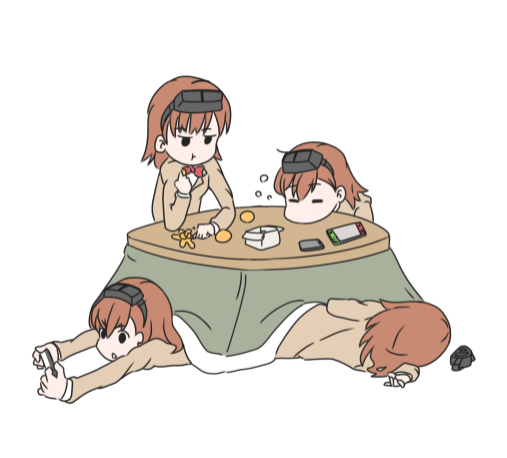
\includegraphics[width=.4\paperwidth]{figures/misaka558.png}
            \end{column}
        \end{columns}
    \end{frame}
    
\end{document}